\documentclass{sigchi}

% Use this command to override the default ACM copyright statement (e.g. for preprints). 
% Consult the conference website for the camera-ready copyright statement.


%% EXAMPLE BEGIN -- HOW TO OVERRIDE THE DEFAULT COPYRIGHT STRIP -- (July 22, 2013 - Paul Baumann)
% \toappear{Permission to make digital or hard copies of all or part of this work for personal or classroom use is 	granted without fee provided that copies are not made or distributed for profit or commercial advantage and that copies bear this notice and the full citation on the first page. Copyrights for components of this work owned by others than ACM must be honored. Abstracting with credit is permitted. To copy otherwise, or republish, to post on servers or to redistribute to lists, requires prior specific permission and/or a fee. Request permissions from permissions@acm.org. \\
% {\emph{CHI'14}}, April 26--May 1, 2014, Toronto, Canada. \\
% Copyright \copyright~2014 ACM ISBN/14/04...\$15.00. \\
% DOI string from ACM form confirmation}
%% EXAMPLE END -- HOW TO OVERRIDE THE DEFAULT COPYRIGHT STRIP -- (July 22, 2013 - Paul Baumann)


% Arabic page numbers for submission. 
% Remove this line to eliminate page numbers for the camera ready copy
% \pagenumbering{arabic}


% Load basic packages
\usepackage{balance}  % to better equalize the last page
\usepackage{graphics} % for EPS, load graphicx instead
\usepackage{times}    % comment if you want LaTeX's default font
\usepackage{url}      % llt: nicely formatted URLs

% llt: Define a global style for URLs, rather that the default one
\makeatletter
\def\url@leostyle{%
  \@ifundefined{selectfont}{\def\UrlFont{\sf}}{\def\UrlFont{\small\bf\ttfamily}}}
\makeatother
\urlstyle{leo}


% To make various LaTeX processors do the right thing with page size.
\def\pprw{8.5in}
\def\pprh{11in}
\special{papersize=\pprw,\pprh}
\setlength{\paperwidth}{\pprw}
\setlength{\paperheight}{\pprh}
\setlength{\pdfpagewidth}{\pprw}
\setlength{\pdfpageheight}{\pprh}

% Make sure hyperref comes last of your loaded packages, 
% to give it a fighting chance of not being over-written, 
% since its job is to redefine many LaTeX commands.
\usepackage[pdftex]{hyperref}
\hypersetup{
pdftitle={Proposal and Survey for a Stock Application},
pdfauthor={Jadees Anton, Connor Hallett, Spencer Lee, Nicolas Lelievre},
pdfkeywords={},
bookmarksnumbered,
pdfstartview={FitH},
colorlinks,
citecolor=black,
filecolor=black,
linkcolor=black,
urlcolor=black,
breaklinks=true,
}

% create a shortcut to typeset table headings
\newcommand\tabhead[1]{\small\textbf{#1}}


% End of preamble. Here it comes the document.
\begin{document}

\title{Proposal and Survey for a Stock Application}
\numberofauthors{4}
\author{
	\alignauthor Jadees Anton\\
		\email{antonj@mcmaster.ca}\\
	\alignauthor Connor Hallett\\
		\email{hallec3@mcmaster.ca}\\
	\alignauthor Spencer Lee\\
		\email{leese5@mcmaster.ca}\\
	\alignauthor Nicolas Lelievre\\
		\email{lelievnm@mcmaster.ca}
}

\maketitle

\begin{abstract}
Be sure to also indicate if you are submitting a DESIGN or RESEARCH project in the ``Abstract'' section of
your submission.
\end{abstract}


\section{Overview}
overview of the topic/software/device of interest – tell me why you want to develop such a system

\section{Design Improvements}
idea of what will be unique/better/improved in your system (versus what already exists – this will be
informed by your software survey)

\section{User Goals}
User goals when using this application are mainly to understand large amounts of information in meaningful ways. Primarily, users are interested in gathering insight related to general stock markets as well as their favourite stocks.



\section{Microsoft Money}
\subsection{Description}
Microsoft's Windows 10 operating system comes bundled with a series of integrated applications, one of which is appropriately named ``Money'' and offers insight pertaining to the stock market, currencies and general finances. The application also enables users to monitor the progress of their favourite stocks as well as read financial articles and calculate mortgage payments.

\subsection{User Tasks}
In order for a user to view general information on the stock market, they must use the \textit{markets} page, listed in the application's sidebar, which displays statistics related to the past and current states of the local and global markets using a simple line graph as well as statistics describing the stocks increases and decreases in value. \\
Users may also view a simplified list of their favourite stocks in their \textit{watchlist}, accessed through the sidebar or the top menu bar, which presents a summary of the stocks to which they have subscribed including current pricing, changes and volume for each stock.

\subsection{Critique}
Although the application does an excellent job of simplifying the interface, it goes beyond and seems to oversimplify it by crowding a lack of relevant information with large amounts of redundant content. For instance, the \textit{home} page's poor visibility shows very little stock ticker information in preference for a myriad of large-tiled articles. \\
The conceptual model of the application is therefore very simplified in terms of usable information as the overcrowded nature significantly decreases its usability. Its severe lack of signifiers also makes finding new stocks and navigating the application challenging, hence decreasing its overall discoverability as users are constantly unsure of what can and cannot be accomplished. \\
It should be noted however that the layout, although crowded at times, is well conceived as the stock information is clear and easily interpreted.



\section{Critique 2}
\subsection{Description}
Brief description of the application.

\subsection{User Tasks}
Identifying tasks the user must perform to achieve their goals.

\subsection{Critique}
How it's bad, bad, bad, good.



\section{HTC Stocks}
\subsection{Description}
HTC Stocks is a mobile Android application that comes installed on all HTC devices.  This app allows the user to add stocks to their list of bookmarked stocks, view basic information about all stocks that they have bookmarked at the same time, and view detailed information about one stock at a time.  The detailed stock view includes a graph of price history, high and low prices, and information about the values at open and close for the stock on the current day.  The application is powered by Yahoo Finance.

%\subsection{User Goals}
%A user of this application will want to quickly view information about a select collection of stocks.  
%They will want to see basic information about all of the stocks that they follow, and detailed information 
%about specific stocks.  The user will also want to maintain their list of favorite stocks, so that the information
%that is displayed to them is the information that they want. 
%finding information about generals stocks and monitoring favorite stocks

\subsection{User Tasks}
For a user to find information about stocks they may be interested in through this application, they first need to add the stock in question to their favorites.  Once this is done, the stock will appear in the users list of favorite stocks, where they can tap on it to see detailed information.\\
To view general information about all of the stocks that a user is following, all that the user needs to do is open the app.  On the home view a list of all of the stocks that a user is currently following is displayed along with the current price of the stock, along with the absolute and relative changes in the stock's price over the trading day.

\subsection{Critique}
This application falls short when it comes to viewing information about stocks that a user may be interested in.  For a user to see any information about a stock, it must be added to their list of favorite stocks.  As a result, the user may end up with a favorites list that is cluttered with stocks that they only wanted to view once, which makes seeing information about their regular stocks more difficult.  This application does a good job however in displaying quick information to the user about their followed stocks.  If the user has maintained an accurate list of their favorite stocks, they will see the majority of the information they need as soon as they open the application.



\section{YAHOO! Finance}
\subsection{Description}
YAHOO! Finance mobile application allows users to track trading prices of current stocks. The application is composed of three main sections: Home, News, and Markets. The Home section contains a list of the user’s stocks that he/she is following, followed by select news articles. The News section contains the latest news reports on various international current events; mostly articles concerning foreign markets and companies. The third section, Markets, allows the user to track the S\&P Composite Index for the Toronto Stock Exchange (TSX), the Dow Jones Industrial Average (DOW), and NASDAQ. 

\subsection{User Tasks}
The first task is for a user to follow a new stock. He/she is first required to open the application. Once on the Home page, the user clicks on the Edit icon, rendering the edit view of the list of the stocks he/she is following. The user then clicks the Add icon and searches for the stock of interest. Once found and selected, the stock is added to the list of followed stocks.\\

The second task is for a user to check which stocks in the American market have increased in the most value in the last day. This can be done by opening the application and going to the Markets page. The user then ensures that the U.S. market button is selected. He/she then scrolls down to the section “Market Gainers” to see which stocks have increased the most in the last day in the American market.


\subsection{Critique}
YAHOO! Finance displays adequate visibility for its overall layout. Intuitively, the Home page contains the most common information that a user would require (status of his/her followed stocks, news items). The News page contains news articles (as expected), and the Markets page contains information regarding each market in an organized fashion. \\

The application lacks organization when displaying its news articles. Like most mobile application, it integrates ads into the user interface. Links to ads appear sporadically in between news articles in the news article feeds on both the Home and News pages. It would make more sense to group all ads together so the user can differentiate an ad from a news article more easily. 


\begin{figure*}
	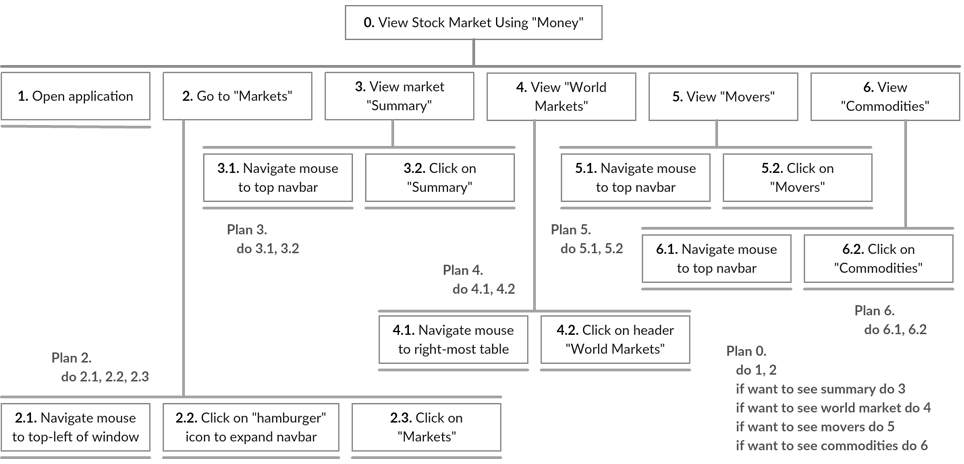
\includegraphics[width=\textwidth]{HTA_1_Money}
	\caption{Viewing stock market HTA and accompanying screen caption of Microsoft Money.}
	\label{fig:figure1}
\end{figure*}

\begin{figure*}
	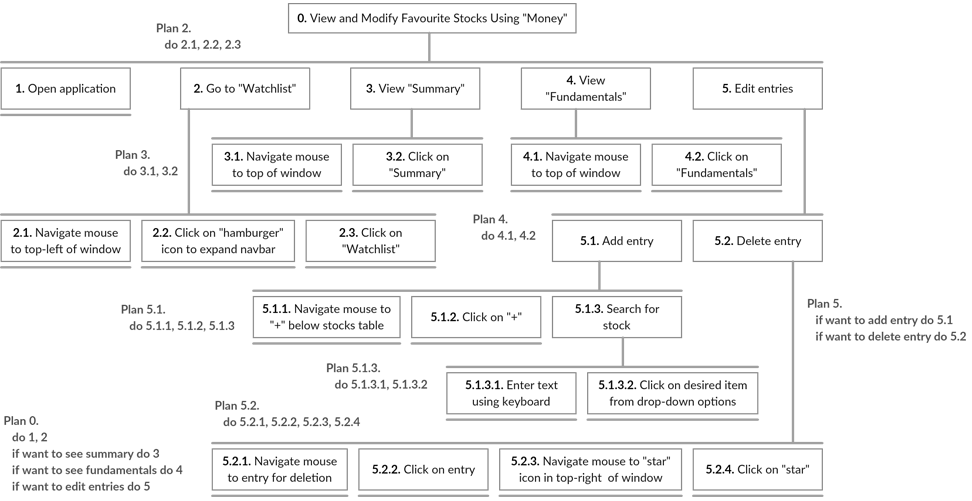
\includegraphics[width=\textwidth]{HTA_2_Money}
	\caption{Viewing and modifying favourite stocks HTA and accompanying screen caption of Microsoft Money.}
	\label{fig:figure2}
\end{figure*}
 


\section{Conclusion}
Paper conclusion (if we have one).




% Balancing columns in a ref list is a bit of a pain because you
% either use a hack like flushend or balance, or manually insert
% a column break.  http://www.tex.ac.uk/cgi-bin/texfaq2html?label=balance
% multicols doesn't work because we're already in two-column mode,
% and flushend isn't awesome, so I choose balance.  See this
% for more info: http://cs.brown.edu/system/software/latex/doc/balance.pdf
%
% Note that in a perfect world balance wants to be in the first
% column of the last page.
%
% If balance doesn't work for you, you can remove that and
% hard-code a column break into the bbl file right before you
% submit:
%
% http://stackoverflow.com/questions/2149854/how-to-manually-equalize-columns-
% in-an-ieee-paper-if-using-bibtex
%
% Or, just remove \balance and give up on balancing the last page.
%
\balance
% REFERENCES FORMAT
% References must be the same font size as other body text.

\bibliographystyle{acm-sigchi}
\bibliography{sample}
\end{document}
